\begin{center}
	\Huge
	Vandrette og lodrette tangenter
\end{center}
\section*{Vandrette og lodrette tangenter}
\stepcounter{section}

Vi ønsker at kunne bestemme de steder, hvor tangenten til parameterkurven for en vektorfunktion $\vv{r}$ er enten lodret eller vandret. Dette er helt analogt til at bestemme toppunkterne for koordinatfunktionerne $x$ og $y$. 

\begin{exa}
	Lad os betragte vektorfunktionen $\vv{r}$ givet ved
	\begin{align*}
		\vv{r}(t) =
		\begin{pmatrix}
			-t^2+1 \\
			-t^3+12t
		\end{pmatrix}.
	\end{align*}
	Vi ønsker at bestemme alle lodrette og vandrette tangenter for denne vektorfunktion. Vi begynder med at bestemme de vandrette tangenter. 
	\begin{align*}
		y'(t) = 0 \ \Leftrightarrow \ -3t^2+12 = 0.
	\end{align*}
	Derfor har parameterkurven for $\vv{r}$ en vandret tangent, når $t=2$ eller $t=-2$. Dette indsættes i $\vv{r}$:
	\begin{align*}
		\vv{r}(2) = 
		\begin{pmatrix}
			-(2)^2+1 \\
			-(2)^3+12\cdot 2
		\end{pmatrix} =
		\begin{pmatrix}
			-3 \\
			16
		\end{pmatrix}.
	\end{align*}
	\begin{align*}
		\vv{r}(-2) =
		\begin{pmatrix}
		-(-2)^2+1 \\
		-(-2)^3+12(-2)
		\end{pmatrix} =
		\begin{pmatrix}
			-3 \\
			-16
		\end{pmatrix}
	\end{align*}
	Parameterkurven for $\vv{r}$ har derfor en vandret tangent i punktet $P_{-2}(-3,-16)$ med ligningen $y=-16$. Den har også en vandret tangent i punktet $P_2(-3,16)$ med ligningen $y=16$. 
	Vi ønsker også at bestemme lodrette tangenter.
	\begin{align*}
		x'(t) = 0 \ \Leftrightarrow \	-2t=0.
	\end{align*}
	Derfor har parameterkurven for $\vv{r}$ en vandret tangent, når $t=0$. Som før indsættes dette i $\vv{r}$.
	\begin{align*}
		\vv{r}(0) = 
		\begin{pmatrix}
			-(0)^2+1 \\
			-(0)^3+12\cdot 0
		\end{pmatrix} =
		\begin{pmatrix}
			1 \\
			0
		\end{pmatrix}
	\end{align*}
	Derfor har parameterkurven for $\vv{r}$ en lodret tangent i punktet $P_0(1,0)$ med ligningen $x=1$.
	På Fig. \ref{fig:tangentgraf} kan en tegning af parameterkurven for $\vv{r}$ ses samt de vandrette og lodrette tangenter. 
	\begin{figure}[H]
		\centering
		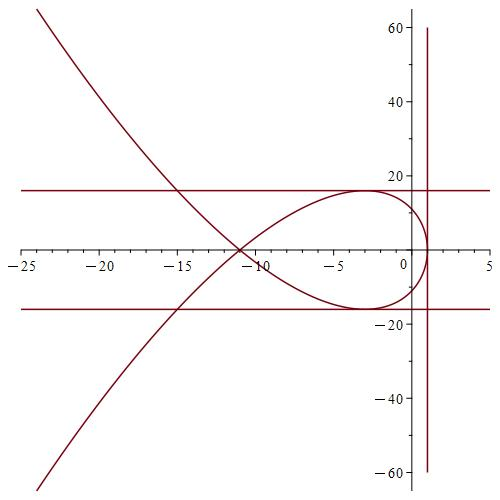
\includegraphics[width=0.7\textwidth]{Billeder/vektortangent.jpg}
		\caption{Lodrette og vandrette tangenter for parameterkurve.}
		\label{fig:tangentgraf}
	\end{figure}
\end{exa}

\section*{Opgave 1}

Bestem de vandrette og lodrette tangenter til følgende vektorfunktioner. Bestem desuden skæringspunktet med tangenten, og tegn vektorfunktionen for at undersøge, om du har fundet de rigtige tangenter.

\begin{align*}
	&1) \  
	\vv{r} =
	\begin{pmatrix}
		t^2 \\
		t^3-24t
	\end{pmatrix}	
	   &2) \ 
	   \vv{r} =
	\begin{pmatrix}
		t^2 \\
		t^3-24t
	\end{pmatrix}    \\
		&3) \  
	\vv{r} =
	\begin{pmatrix}
		\ln(t)-t^2 \\
		t^3-3t^2
	\end{pmatrix}	
	   &4) \ 
	   \vv{r} =
	\begin{pmatrix}
		\cos(t) \\
		\sin(t)
	\end{pmatrix}    \\
\end{align*}

\section*{Opgave 2}

Lav aflevering.